\newpage
\chapter{Anhang}
%\addcontentsline{toc}{chapter}{Anhang}

%	\section{Vom Telefon zum Smartphone}
% 		\subsection{Entstehungsgeschichte}
% 		
%  		Die Geschichte des Telefons beginnt mit Alexander Graham Bell im Jahre 1876,
% 		dem Jahr in dem er das von Ihm entwickelte elektromagnetische Telefon zum
% 		ersten Mal au�erhalb seines Labors, in Boston, auf einer Versuchsstrecke von
% 		8,5 Km L�nge angewandt hat. Bell stellt sein verbessertes Telefon vor. Er
% 		l�sst es am 08. M�rz patentieren. 
% 		
% 		Einige Zeit sp�ter begann die Entwicklung des Mobilfunks. 1926 stellt die
% 		Deutsche Reichsbahn und Reichspost einen Telefondienst auf der Strecke
% 		zwischen Hamburg und Berlin zur Verf�gung, der Reisenden der 1. Klasse
% 		angeboten wird.
% TODO: evtl. in den Anhang? oder ganz raus... eigentlich irrelevant!


\section{Jailbreak}
%TODO: ausf�rhlichere Erkl�rung + Bilder

WIKIPEDIA

Seit dem 27. Juli 2010 ist die Entsperrung in den USA legal, die Rechtslage in
Deutschland ist bisher nicht eindeutig gekl�rt. 

Im Juli 2007 beschrieb der Norweger Jon Lech Johansen in seinem Blog, wie man
die Funktionen des iPhones auch ohne AT\&T-Vertrag nutzen kann.

Im August 2007 berichtete das Technik-Blog Gizmodo, dass sich das iPhone mit
Hilfe einer sogenannten ``Turbo-SIM-Karte'' auch in anderen GSM-Netzen betreiben
lasse. Am 6. September 2007 ver�ffentlichte die Webseite des APC Magazine
eine Zehn-Schritte-Anleitung zur Nutzung des iPhones in weltweit allen
GSM-Netzen mit Hilfe einer Turbo-SIM-Karte.

Ebenfalls im August 2007 gelang es dem US-Amerikaner George Hotz, ohne den
Umweg �ber eine Turbo-SIM-Karte die Beschr�nkung der Nutzung seines iPhones
auf das AT\&T-Netz aufzuheben. In seinem Blog beschrieb er dazu ein Verfahren,
das komplizierte Eingriffe in die Hardware erfordert.

Im September 2007 stellte das iPhone Dev Team, eine freie Gruppe von
Programmierern, eine Software-Netlock-Entsperrung f�r das iPhone frei im
Internet zur Verf�gung. Damit war das iPhone weltweit in allen GSM-Netzen auch
f�r iPhone-Besitzer nutzbar, die den technischen Aufwand bislang verf�gbarer
komplizierter Hacks gescheut hatten.

Einen Tag nach Release des iPhones 3GS wurde ein Tool zur Entsperrung dieses
Ger�tes ver�ffentlicht.

Am 22. Juni 2009 hat das iPhone Dev-Team eine rein softwarebasierte
SIM-Entsperrung namens ultrasn0w f�r alle iPhones ab Firmware 3.0
ver�ffentlicht, mit der die Ger�te in allen Netzen betrieben werden k�nnen.
Mit vielen Firmwarereleases kommen neue Versionen der Netzkontrollsoftware,
wodurch neue Exploits gefunden werden m�ssen, um diese erneut freizuschalten.
Bisher ist dies f�r jedes Baseband gelungen. Im Mai 2010 wurde das Tool Spirit
ver�ffentlicht, das auch f�r das iPad mit iOS 3.2 funktioniert.

Am 1. August 2010 wurde ein webbasierter Jailbreak namens JailbreakMe
ver�ffentlicht, mit dem auch das iPhone 4 ge�ffnet werden kann. Hierf�r wurde
ein Programmfehler bei der PDF-Darstellung im Programm Mobile Safari genutzt.
Am Tag darauf warnte das BSI davor, mit dem iPhone PDFs zu �ffnen, da auch ein
sch�dlicher Code ausgef�hrt werden k�nnte. Eine Apple-Pressesprecherin
verk�ndete, dass Apple den Fehler bereits behoben habe und schnellstm�glich
ein Update herausbringen werde.

Apple gab daraufhin am 11. August 2010 ein Update (iOS 4.0.2) heraus, das zwei
Sicherheitsl�cken schloss. Die eine L�cke betraf eine Systembibliothek
(``Freetype'') - durch die zweite erreichte das ausf�hrende Programm
System-Rechte am Ger�t.

\section{Hackint0sh}
%TODO: ausf�rhlichere Erkl�rung + Bilder

\section{Model-View-Controller-Prinzip}
%TODO: Erkl�rung + Bilder





% \clearpage
% \thispagestyle{empty}
% \begin{figure}[hp]
% 
\includegraphics[width=\textwidth]{beispiel}
% \end{figure} 
% \clearpage
% 
% \chapter{Beispielanhang 2}
% Dies ist das Deckblatt. Es sollte die kurze Beschreibung der n�chsten Seite enthalten. Der Titel ist meist ausreichend.
% 
% % so gehts auch
% \clearpage
% \thispagestyle{empty}
% \begin{figure}[hp]
% 
\includegraphics[height=\textwidth,angle=90]{beispiel}	% jetzt querformat
% \end{figure} 
% \clearpage
% 
% \addtocontents{toc}{\vspace{-1ex}}
% \chapter{Beispielanhang 3}
% Dies ist das Deckblatt. Es sollte die kurze Beschreibung der n�chsten Seite enthalten. Der Titel ist meist ausreichend.
% 
% 
% % Wenn der Anhang als PDF vorliegt kann man ihn einfach so einf�gen: (Paket pdfpages n�tig)
% \ifpdf % funktioniert leider nur mit pdfLaTeX 
% 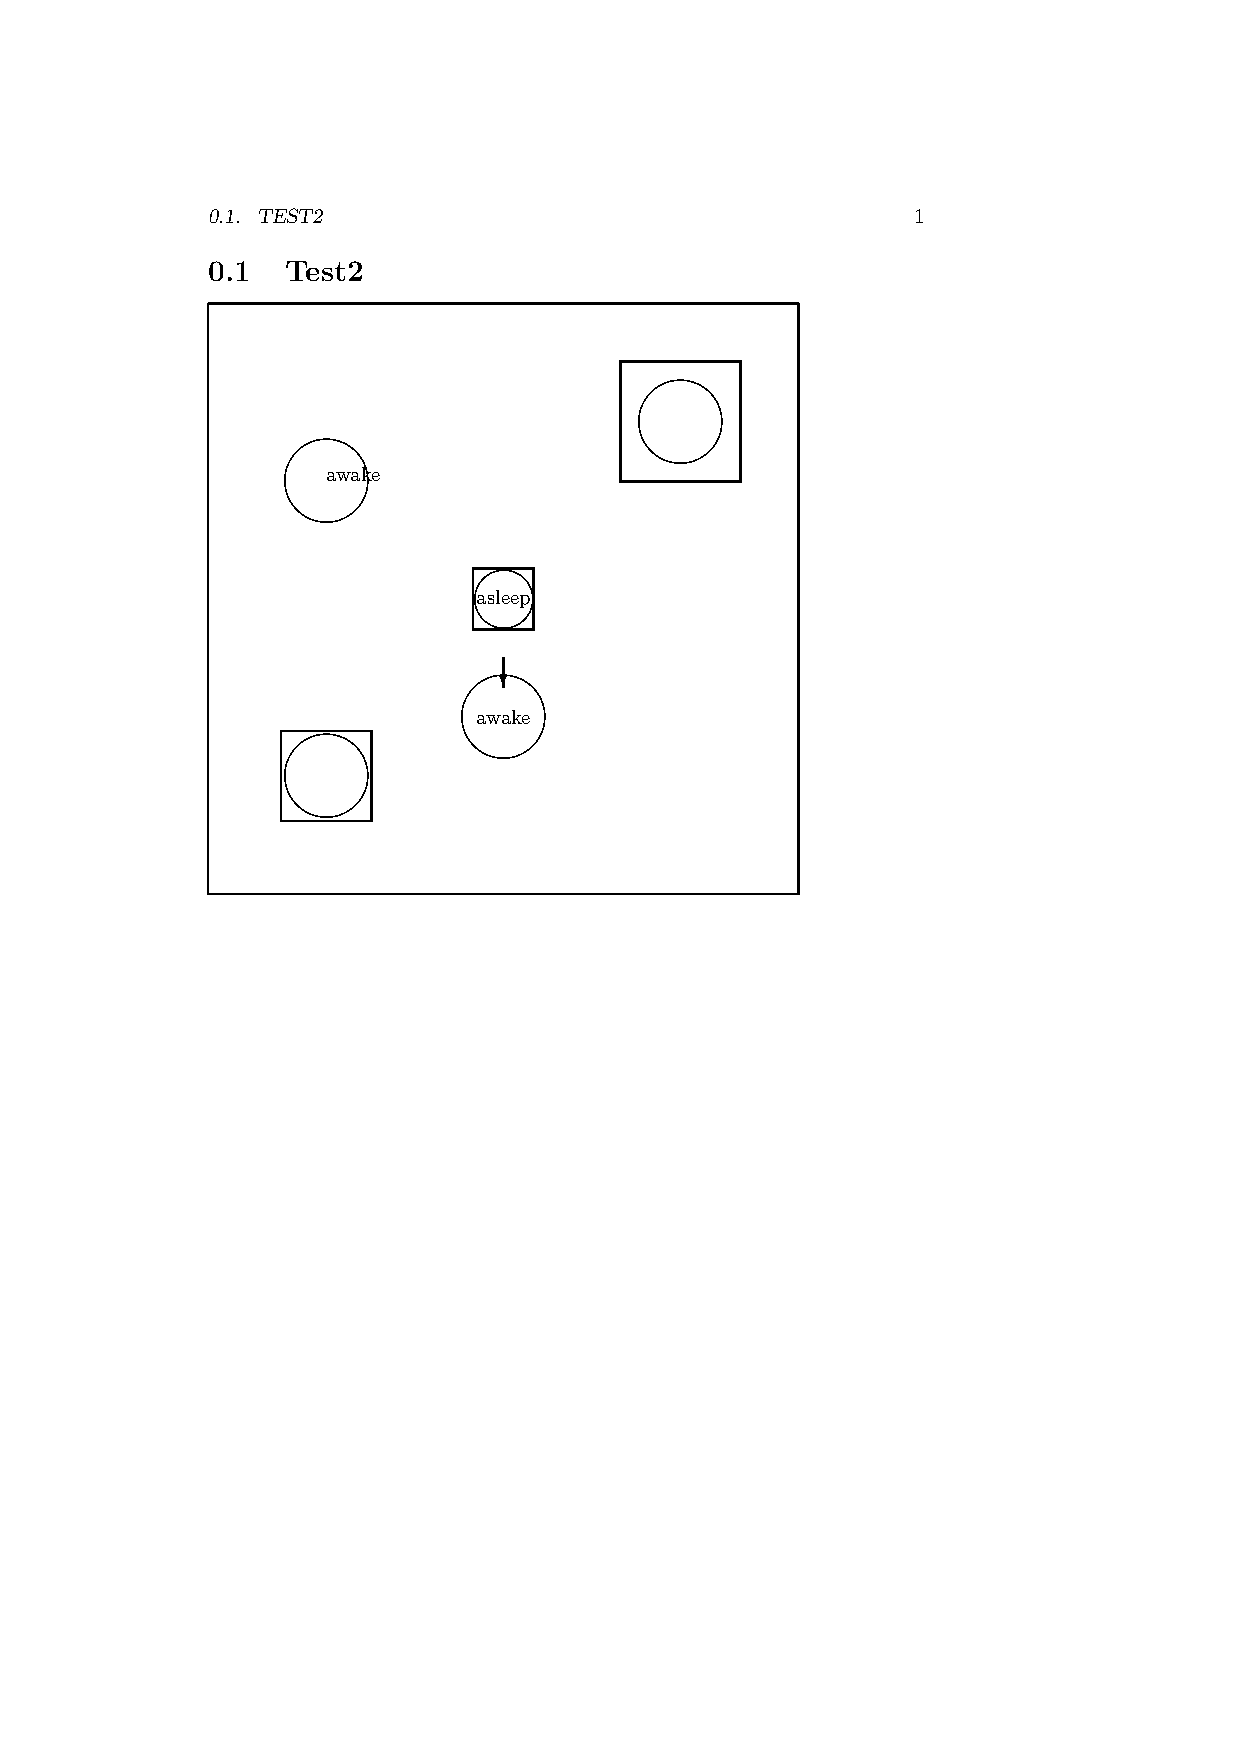
\includepdf[pages=-]{anhang/beispielanhang}	% pages=- bedeutet: alle Seiten | Wie bei Bilder die Dateierweiterung (.pdf) am besten weglassen
% % Weites Beispiel: Nur Seiten 1-2 und 4, Papier querformat mit 2 Seiten pro Seite
% %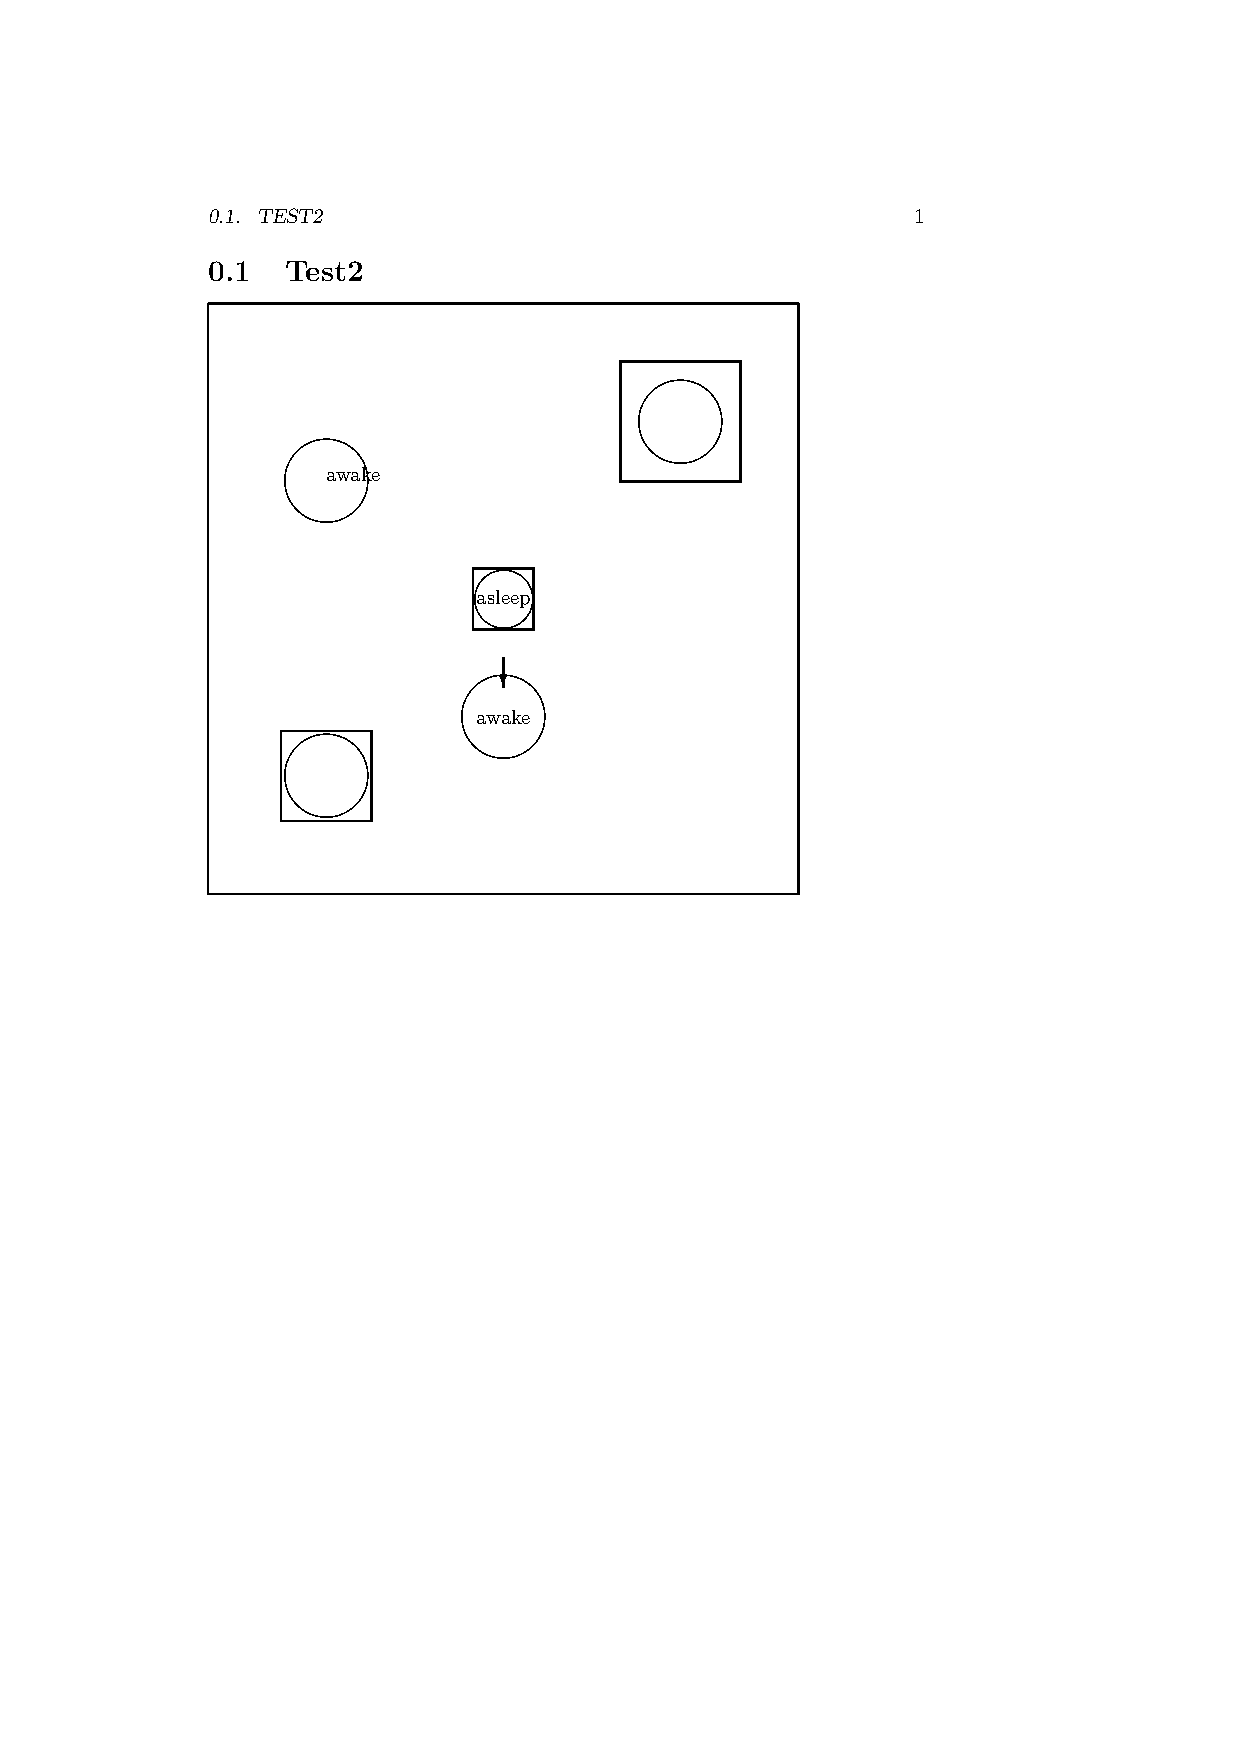
\includepdf[pages={1-2,4},landscape,nup=1x2]{anhang/beispielanhang}
% 
% \else  % bei der Verwendung vom normalen LaTeX:
% \newpage
% \addtocounter{page}{5}	% Seitenz�hler hochz�hlen und Anhang nach dem Drucken manuell hinzuf�gen
% % Hier wurde angenommen, dass der Anhang f�nf Seiten lang ist
% \fi
% 
% \chapter{Weiterer Anhang}
